\section{1.2 Shorter and shorter}
We are tasked with creating a filter for which the specification has been partly destroyed by a coffee addict.
Luckily, the surviving information is sufficient to create the original information.

The filter should pass all frequencies between 0 and 5kHz with a gain on 0dB, this means the filter is a lowpass filter.
As we can see from the sketched frequency response, 5kHz corresponds to one sixth of the sampling frequency since a 
normalised frequency of 1 corresponds to the nyquist frequency. The sampling frequency is 30kHz. 
Additionally the impulse response of the filter should be 601 samples long, meaning our filter is of the 600th order
as it is a FIR filter where the length of the impulse response is \(N+1\) where \(N\) is the order of the filter.

\begin{figure}
	\center
	\includegraphics{./picture/ha9_1_2_1.eps}
	\caption{Impulse response of the 600th order FIR filter created by sampling a perfect lowpass filter in the frequency domain
	and transforming back to the time domain. It is a time-shifted sampled sinc function.}
	\label{fig:1_2_ir}
\end{figure}

The filter can be constructed in Matlab using the frequency domian equivalence method. This means we construct a 
perfect lowpass filter in the frequency domain, and sample it at the frequency bins given by our signal length.
Our signal is 601 samples long, which at 30kHz yields a period of 0.02 seconds, meaning that bins in the frequency
domain are separated by 50Hz. After sampling our perfect lowpass filter, we transform back to the time domain and delay by \(\frac{N-1}{2}\) samples, 
obtaining the impulse response shown in figure~\ref{fig:1_2_ir} which is, not surprisingly, a time-shifted sinc function.


Since we want to please our boss, we decide to try minimizing the resources required to implement the filter. We do this by
reducing the length of the impulse response and applying an appropriate window to reduce high-frequency components. We 
choose to use the hamming filter, applied to impulse responses of varying lengths shown in figure~\ref{fig:1_2_freq}. 
In the end we conclude that the filter with an impulse response length of 201 samples is actually better when windowed than
the original impulse response in terms of rolloff without sacrificing any significant gain in the passband.

\begin{figure}
	\center
	\includegraphics{./picture/ha9_1_2_2.eps}
	\caption{Frequency reponse of the *original impulse response as well as the impulse responses reduced in length by windowing
		with a hamming window.
		Legend shows the length of the impulse response in samples. It is clear that the windowed impulse responses have better
		maximum attenuation all the way to down to 11 samples, however the rolloff is worse for impulse responses shorter than 300 
		samples.
		Beyond 51 samples the filter behaviour is completely unsatisfactory for our purposes. 201 would be the best compromise
		between performance and cost.
		Note that the phase is linear until the cutoff frequency after which the sawtooth pattern is caused by the inability to
		represent small changes with floating point numbers at those magnitudes.
	}
	\label{fig:1_2_2}
\end{figure}
